\documentclass[conference]{IEEEtran}
\IEEEoverridecommandlockouts
% The preceding line is only needed to identify funding in the first footnote. If that is unneeded, please comment it out.
\usepackage{cite}
\usepackage{amsmath,amssymb,amsfonts}
\usepackage{algorithmic}
\usepackage{graphicx}
\usepackage{textcomp}
\usepackage{xcolor}
\usepackage[utf8]{inputenc}
\usepackage[T1]{fontenc}
\usepackage[vietnamese]{babel}

\def\BibTeX{{\rm B\kern-.05em{\sc i\kern-.025em b}\kern-.08em
    T\kern-.1667em\lower.7ex\hbox{E}\kern-.125emX}}
\begin{document}

\title{Tạo sinh chú thích ảnh với cơ chế chú ý\\
{\footnotesize Trường Đại Học Khoa Học Tự Nhiên, thành phố Hồ Chí Minh, Việt Nam\\}
}

\author{\IEEEauthorblockN{21120127 Lê Hoàng Sơn}
\IEEEauthorblockA{\textit{VNUHCM} \\
\textit{HCMUS}\\
tp Hồ Chí Minh, Việt Nam \\
21120127@student.hcmus.edu.vn}
\and
\IEEEauthorblockN{21120085 Võ Gia Khang}
\IEEEauthorblockA{\textit{VNUHCM} \\
\textit{HCMUS}\\
tp Hồ Chí Minh, Việt Nam \\
21120085@student.hcmus.edu.vn}
}

\maketitle

\begin{abstract}
Tài liệu này mô tả xây dựng và huấn luyện mô hình phát sinh chú thích ảnh có chú ý. Mô hình này được xậy dựng dựa trên kiến trúc Encoder, Decoder và Attention Mechanism trên tập dữ liệu Flickr8k. Bên cạch đó, chúng ta sẽ thử nghiệm cải tiến mô hình.
\end{abstract}

\begin{IEEEkeywords}
Show, Tell, and Attend: Image Captioning with Attention Mechanism
\end{IEEEkeywords}

\section{Giới thiệu}
Chú thích hình ảnh nhằm mục đích tự động tạo ra các câu mô tả cho hình ảnh, chụp các đối tượng và mối quan hệ của chúng. Nhiệm vụ đầy thách thức này kết nối Thị giác máy tính (CV) và Xử lý ngôn ngữ tự nhiên (NLP) trong Trí tuệ nhân tạo (AI).
Những tiến bộ gần đây, chẳng hạn như các mô hình dựa trên sự chú ý, đã tạo ra những kết quả mạnh mẽ, cho phép các ứng dụng như công cụ trợ năng và gắn thẻ nội dung. Trong dự án này, chúng tôi triển khai một mô hình chú thích hình ảnh bằng cách sử dụng khuôn khổ CNN-RNN với sự chú ý trực quan, lấy cảm hứng từ 'Show, Attend and Tell' và tinh chỉnh nó trên tập dữ liệu Flickr8k để cải thiện chất lượng chú thích trong hơn 6 tuần.\\
Bài toán có thể được mô tả như sau: Cho ảnh đầu vào với 03 kênh màu RGB, mô hình sẽ tạo ra một câu mô tả cho ảnh đó bằng ngôn ngữ Tiếng Anh và ở hiện tại đơn. Ví dụ, ảnh đầu vào "chú chó với nền cỏ xanh" thì mô hình sẽ có thể tạo sinh ra chú thích mô tả ngắn gọn "A dog sits on green grass".\\

\section{Công trình liên quan}

\subsection{Show, Attend and Tell}
Show, Attend and Tell \cite{show_attend_tell} giới thiệu cơ chế chú ý cho phép mô hình tập trung vào các vùng quan trọng của hình ảnh. Mô hình sử dụng kiến trúc CNN (encoder) và LSTM (decoder) với cơ chế chú ý trực quan, cho phép nó tự học cách tập trung vào các phần liên quan của hình ảnh khi tạo ra từng từ trong chú thích.

\subsection{A PyTorch Tutorial to Image Captioning}
Một triển khai thân thiện với người mới bắt đầu cho mô hình chú thích hình ảnh bằng PyTorch \cite{pytorch_tutorial} cung cấp cách thực hiện CNN + LSTM với cơ chế chú ý. Dự án này sử dụng tập dữ liệu Flickr8k/COCO và cung cấp mã nguồn mở, hướng dẫn chi tiết giúp hiểu rõ quy trình xây dựng mô hình chú thích hình ảnh.

\subsection{Show and Tell}
Show and Tell \cite{show_tell} là mô hình sớm hơn sử dụng kiến trúc CNN + LSTM không có cơ chế chú ý. Đây được coi là mô hình cơ sở để so sánh hiệu quả của các mô hình sau này có tích hợp cơ chế chú ý. Mô hình này đã đặt nền tảng cho các phương pháp tiên tiến hơn trong lĩnh vực chú thích hình ảnh tự động.

% Cần thêm các tham chiếu sau vào phần tài liệu tham khảo
% \bibitem{show_attend_tell} K. Xu et al., "Show, Attend and Tell: Neural Image Caption Generation with Visual Attention," arXiv:1502.03044, 2015.
% \bibitem{pytorch_tutorial} S. G. Vinod, "A PyTorch Tutorial to Image Captioning," GitHub repository, 2018.
% \bibitem{show_tell} O. Vinyals et al., "Show and Tell: A Neural Image Caption Generator," arXiv:1411.4555, 2014.

\section{Phương pháp}
\subsection{Mô hình}
\begin{figure}[htbp]
    \centering
    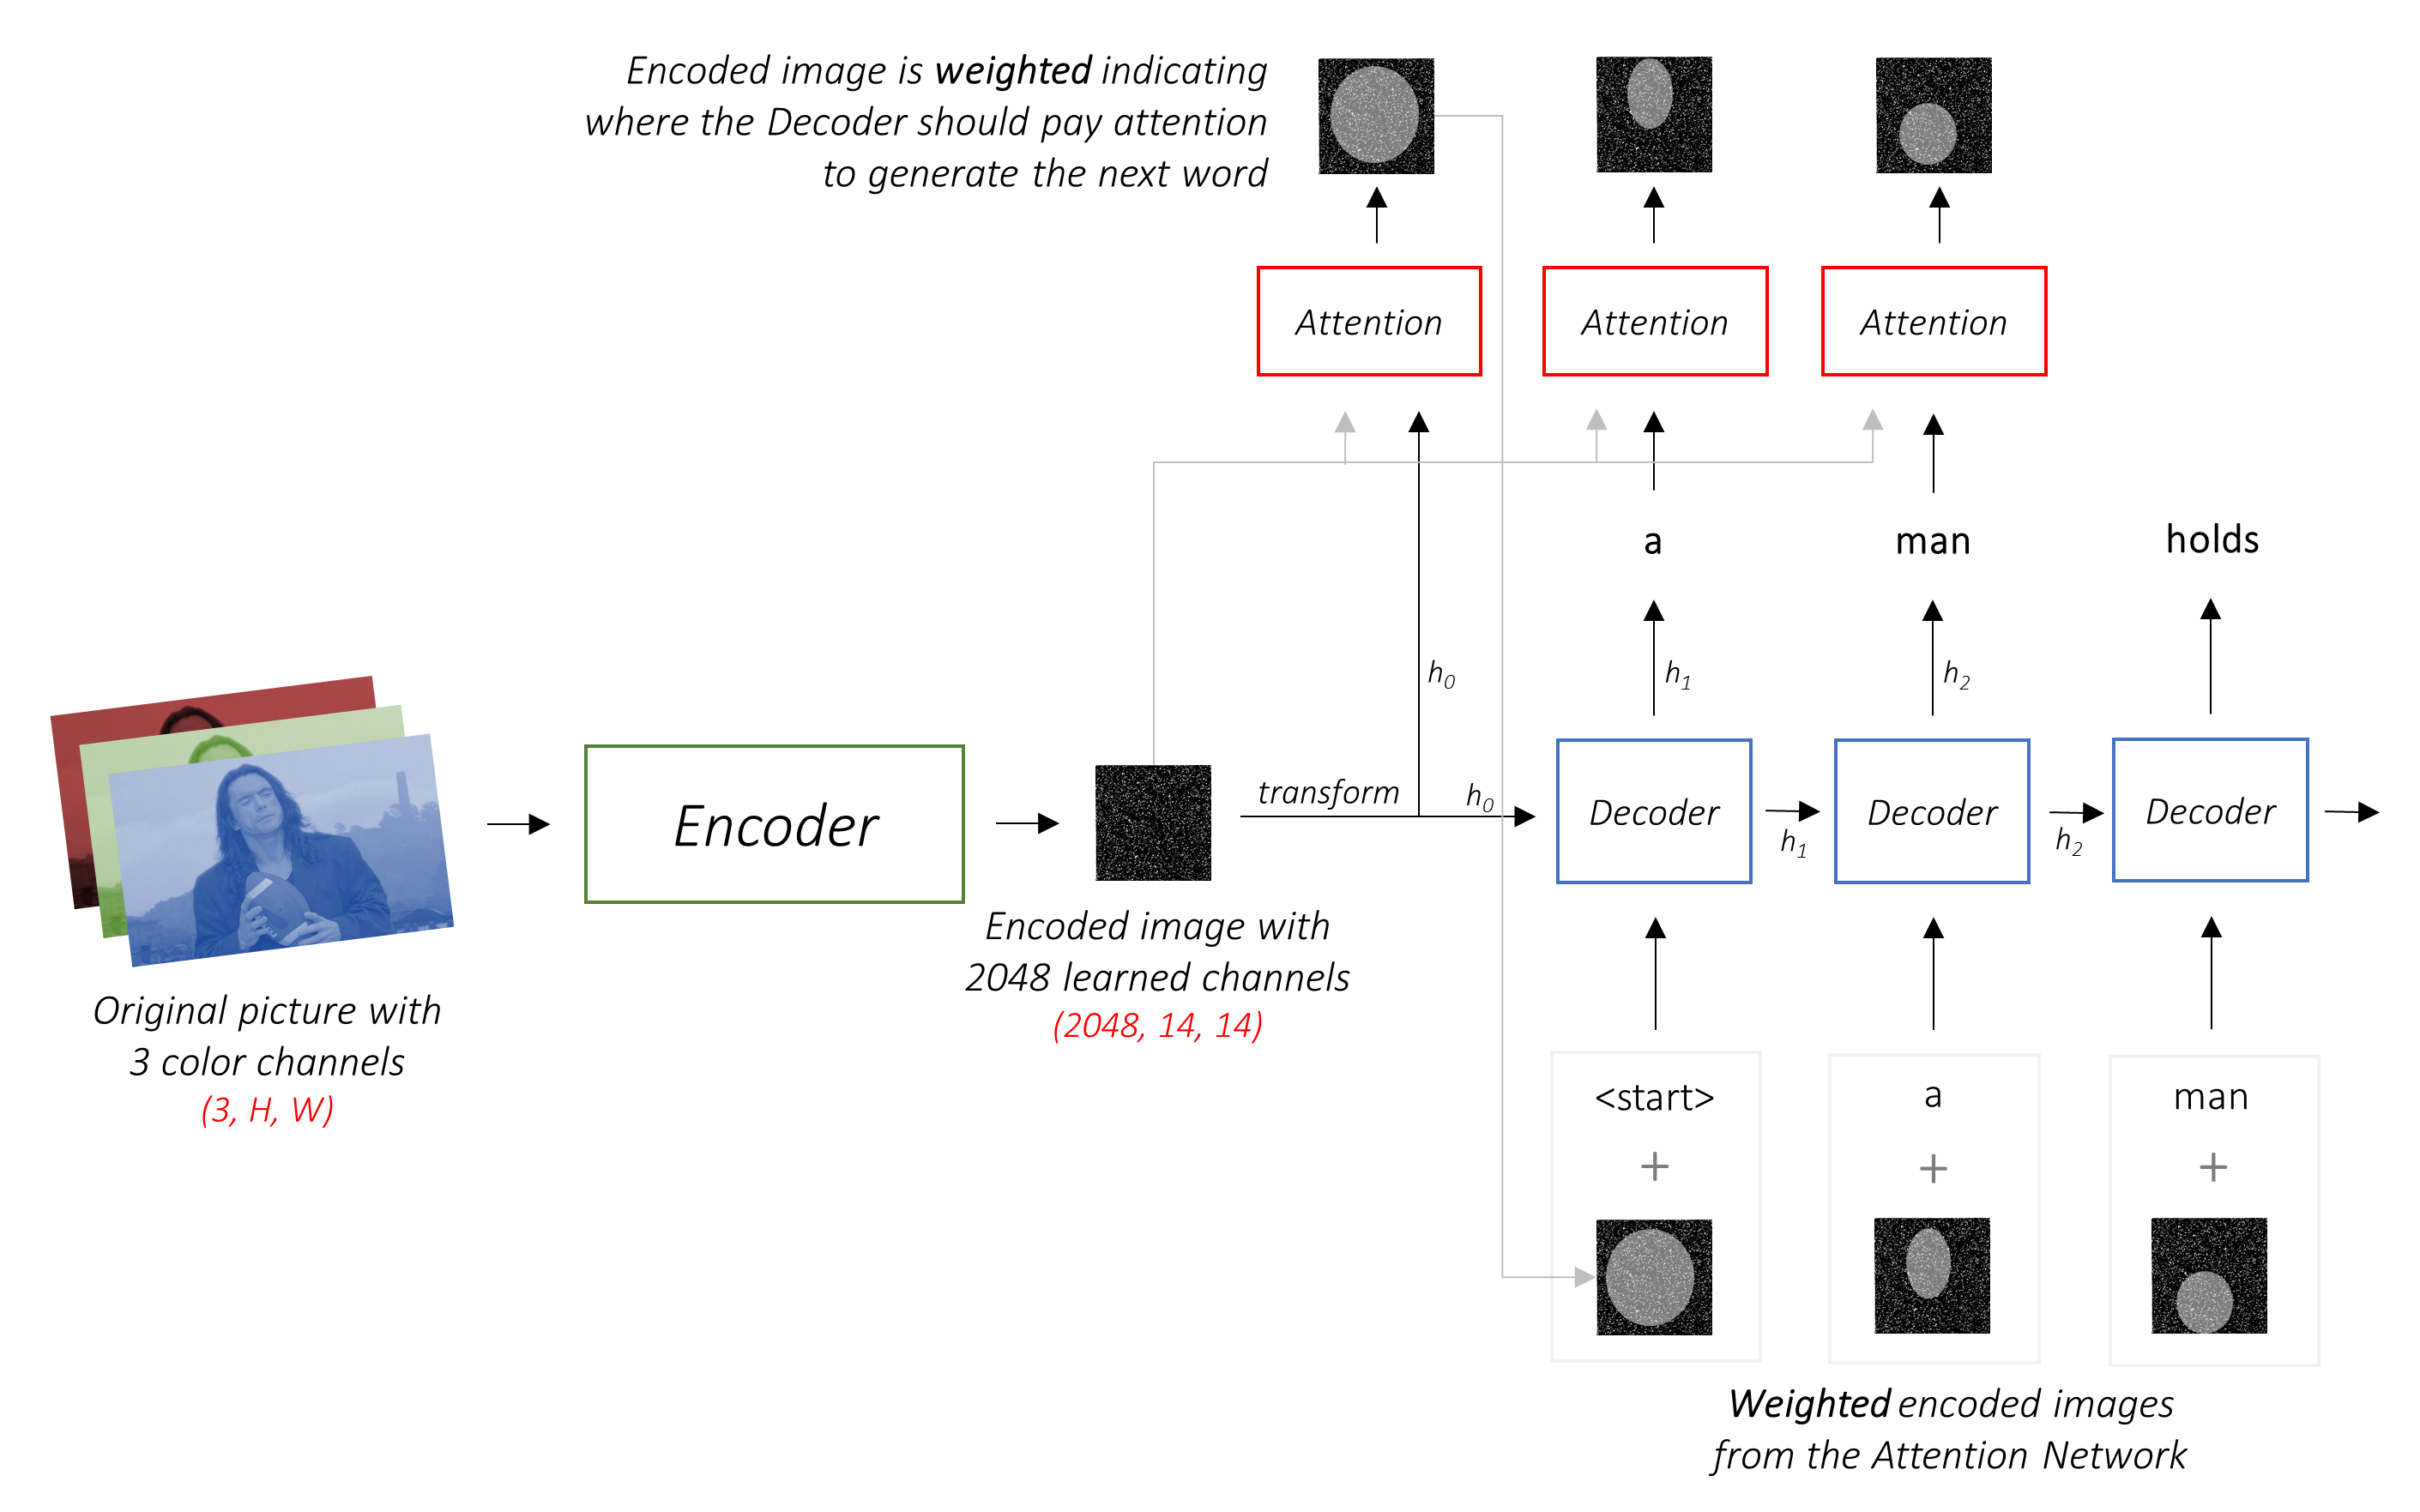
\includegraphics[width=\linewidth]{attachments/model.png}
    \caption{Kiến trúc tổng thể của mô hình Image Captioning với cơ chế chú ý, bao gồm Encoder CNN (ResNet-101), cơ chế Attention và Decoder LSTM.}
    \label{fig:model}
\end{figure}
\subsubsection{Encoder}
Chúng tôi sẽ sử dụng một mạng CNN để trích xuất đặc trưng từ ảnh đầu vào. Các đặc trưng này sẽ được sử dụng trong cơ chế chú ý và bộ giải mã để tạo ra mô tả.\\
Ở đây chúng tôi sẽ sử dụng ResNet-101 để trích xuất đặc trưng từ ảnh. ResNet-101 là một mạng nơ-ron tích chập sâu với 101 lớp, giúp cải thiện khả năng học và giảm thiểu vấn đề biến mất gradient. Chúng tôi sẽ sử dụng các lớp cuối cùng của ResNet-101 để lấy đặc trưng cho ảnh đầu vào.

\subsubsection{Attention}
Cài đặt cơ chế chú ý bằng các lớp tuyến tính đơn giản để mô hình học cách tập trung vào các phần quan trọng của ảnh khi tạo từng từ.

\subsubsection{Decoder}
Sử dụng Long Short-Term Memory (LSTM) để tạo ra câu mô tả từ các đặc trưng đã được trích xuất và thông tin chú ý.

\subsection{Hàm mất mát}
Hàm mất mát được sử dụng trong mô hình này là hàm mất mát chéo entropy, giúp đo lường sự khác biệt giữa phân phối xác suất dự đoán và phân phối xác suất thực tế. Hàm mất mát này sẽ được tối ưu hóa trong quá trình huấn luyện để cải thiện độ chính xác của mô hình.

\subsection{Đánh giá BLEU}

Đánh giá mô hình sẽ được thực hiện bằng cách sử dụng chỉ số BLEU, một phương pháp phổ biến để đo lường chất lượng của các mô tả được tạo ra so với các mô tả tham chiếu. Chỉ số BLEU sẽ giúp chúng tôi đánh giá độ chính xác và tính tự nhiên của các câu mô tả.


\section{Kế hoạch}
\subsection{Tổng quan}
Dự án này được thực hiện trong khoảng thời gian 6 tuần, trong đó chúng tôi lập kế hoạch triển khai và cải tiến mô hình chú thích hình ảnh dựa trên kiến trúc Encoder-Attention-Decoder.
\subsection{Kiến trúc đề xuất}
Mô hình của chúng tôi sẽ sử dụng kiến trúc tương tự như "Show, Attend and Tell":
\begin{itemize}
    \item \textbf{Encoder}: Sử dụng Convolutional Neural Network (ResNet-101) để trích xuất đặc trưng từ ảnh, tạo ra L vector đại diện cho các phần khác nhau của ảnh, mỗi vector có chiều D.
    \item \textbf{Attention}: Cài đặt cơ chế chú ý bằng các lớp tuyến tính đơn giản để mô hình học cách tập trung vào các phần quan trọng của ảnh khi tạo từng từ.
    \item \textbf{Decoder}: Sử dụng Long Short-Term Memory (LSTM) để tạo ra câu mô tả từ các đặc trưng đã được trích xuất và thông tin chú ý.
\end{itemize}

\subsection{Tiến độ thực hiện}
\begin{itemize}
    \item \textbf{Tuần 1-2}: Thu thập và tiền xử lý dữ liệu Flickr8k, xây dựng pipeline dữ liệu
    \item \textbf{Tuần 3-4}: Cài đặt mô hình cơ bản (Encoder-Decoder) không có cơ chế chú ý
    \item \textbf{Tuần 4-5}: Tích hợp cơ chế chú ý và tối ưu hóa mô hình
    \item \textbf{Tuần 5-6}: Đánh giá mô hình sử dụng BLEU score và thực hiện cải tiến
\end{itemize}

\subsection{Cải tiến dự kiến}
\begin{itemize}
    \item Thử nghiệm với các mạng CNN khác nhau cho Encoder (ResNet, Inception-v3)
    \item Tích hợp beam search để cải thiện chất lượng mô tả được tạo ra
    \item Fine-tuning encoder để nâng cao hiệu suất của mô hình
    \item So sánh hiệu quả giữa mô hình có cơ chế chú ý và không có cơ chế chú ý
\end{itemize}

\section{Huấn luyện và phân tích mô hình}
\subsection{Mô tả bộ dữ liệu}

Dữ liệu được sử dụng trong mô hình này là tập dữ liệu Flickr8k, bao gồm 8,000 hình ảnh và các mô tả tương ứng. Tập dữ liệu này được chia thành các phần huấn luyện, kiểm tra và xác thực để đảm bảo mô hình có thể học và đánh giá hiệu quả.\\
Tuy nhiên, ở đây chúng tôi sẽ sử dụng bộ mô tả ảnh của Andrej Karpathy \cite{pytorch_tutorial} với 8,000 hình ảnh và 40,000 mô tả. Mỗi hình ảnh có 5 mô tả khác nhau, giúp mô hình học được nhiều cách diễn đạt khác nhau cho cùng một nội dung.\\
Để chuẩn bị dữ liệu cho mô hình, chúng tôi đã thực hiện các bước sau:
\begin{itemize}
    \item Xây dựng Worldmap, ánh xạ các từ trong mô tả thành các chỉ số số nguyên.
    \item Tổ chức dữ liệu thành tập huân luyện và kiểm tra dưới định dạng hdf5 để dễ dàng truy cập và xử lý.
    \item Thêm từ đặc biệt như <start> và <end> để đánh dấu bắt đầu và kết thúc của một mô tả.
\end{itemize}

\subsection{Các siêu tham số}

\begin{itemize}
    \item Learning rate: 0.001
    \item Batch size: 32
    \item Number of epochs: Do bị giới hạn về thời gian và không thể chạy trên GPU, chúng tôi sẽ dừng lại ở epoch 5.
    \item Optimizer: Adam
\end{itemize}

\section{Kết luận}

\begin{thebibliography}{00}
\bibitem{show_attend_tell} K. Xu et al., "Show, Attend and Tell: Neural Image Caption Generation with Visual Attention," arXiv:1502.03044, 2015.
\bibitem{pytorch_tutorial} S. G. Vinod, "A PyTorch Tutorial to Image Captioning," GitHub repository, 2018.
\bibitem{show_tell} O. Vinyals et al., "Show and Tell: A Neural Image Caption Generator," arXiv:1411.4555, 2014.
\end{thebibliography}
\vspace{12pt}
\color{red}

\end{document}